\documentclass{beamer}
\usepackage[T1]{fontenc}
%\usepackage{arevtext,arevmath}
%\usepackage{ccfonts} 
\usepackage[utf8]{inputenc}
%\usepackage[italian]{babel}
\usetheme{Rochester}
\usefonttheme[onlymath]{serif}
\usepackage{diffcoeff}
\usepackage{graphicx}
\usepackage{bm}
\usepackage{amsmath}
\usepackage{amssymb}
\usepackage{wrapfig}
\usepackage{amsfonts}
\usepackage{amsthm}
\usepackage{amscd}
\usepackage{multicol}
\usepackage{tikz}
\newenvironment{sistema}%
{\left\lbrace\begin{array}{@{}l@{}}}%
{\end{array}\right.}

\title{Modelling genetic dynamical data using stochastic dynamical systems on
graphs}%\author{Riccardo Scheda \\ %\flushleft{Relatore: Prof. Armando Bazzani}}
\institute[]{\\PhD Application in Data Science and Computation - Università di Bologna}
\author{\Large{Riccardo Scheda}}
%\date{Luglio 2020}


\begin{document}

\begin{frame}
\maketitle
\end{frame}


\begin{frame}
\frametitle{Introduction - Gene Regulatory Networks}
\begin{enumerate} 
\item Gene Regulatory Networks in cellular processes:
\begin{enumerate}[] \item cell  differentiation \item metabolism \item signal  transduction
\end{enumerate}
\item GRNs are the focus of the research in systems biology
\item huge amount of genetic data

\end{enumerate}
\begin{figure}[h]
\centering
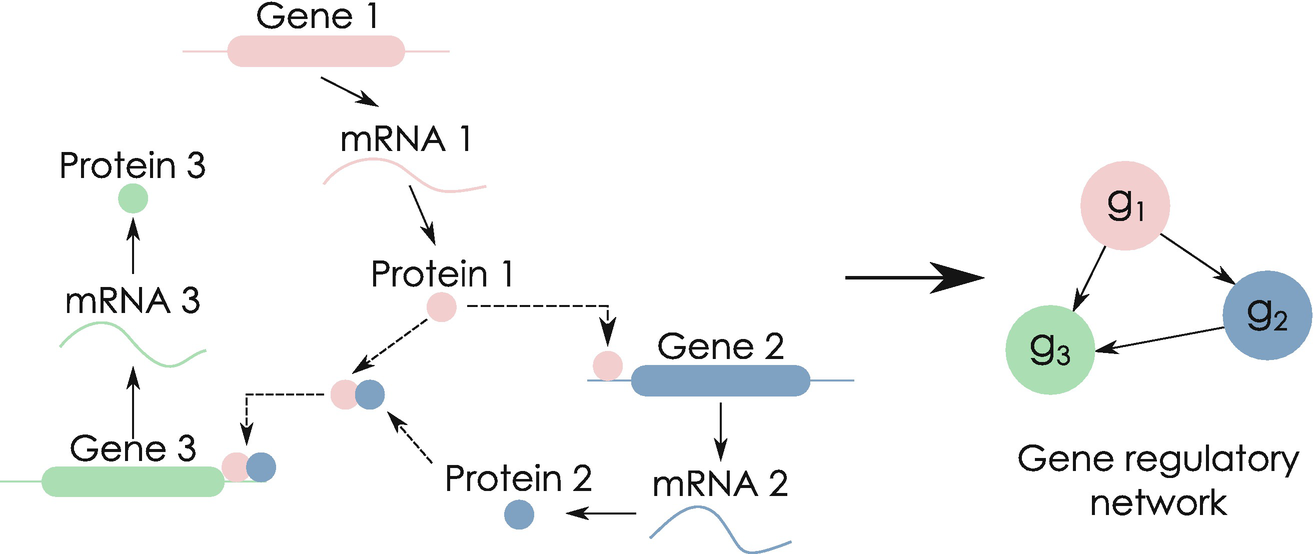
\includegraphics[scale=0.5]{GRN.png}
\end{figure}
\end{frame}


\begin{frame}
\frametitle{Big Data -  GRNs}
GRNs in Data Science:
\begin{enumerate}
\item Huge amount of data from gene expression measurements
\item heterogeneous data (different cells, proteins, etc)
\item dynamical data
\end{enumerate}

\begin{figure}[h]
\centering
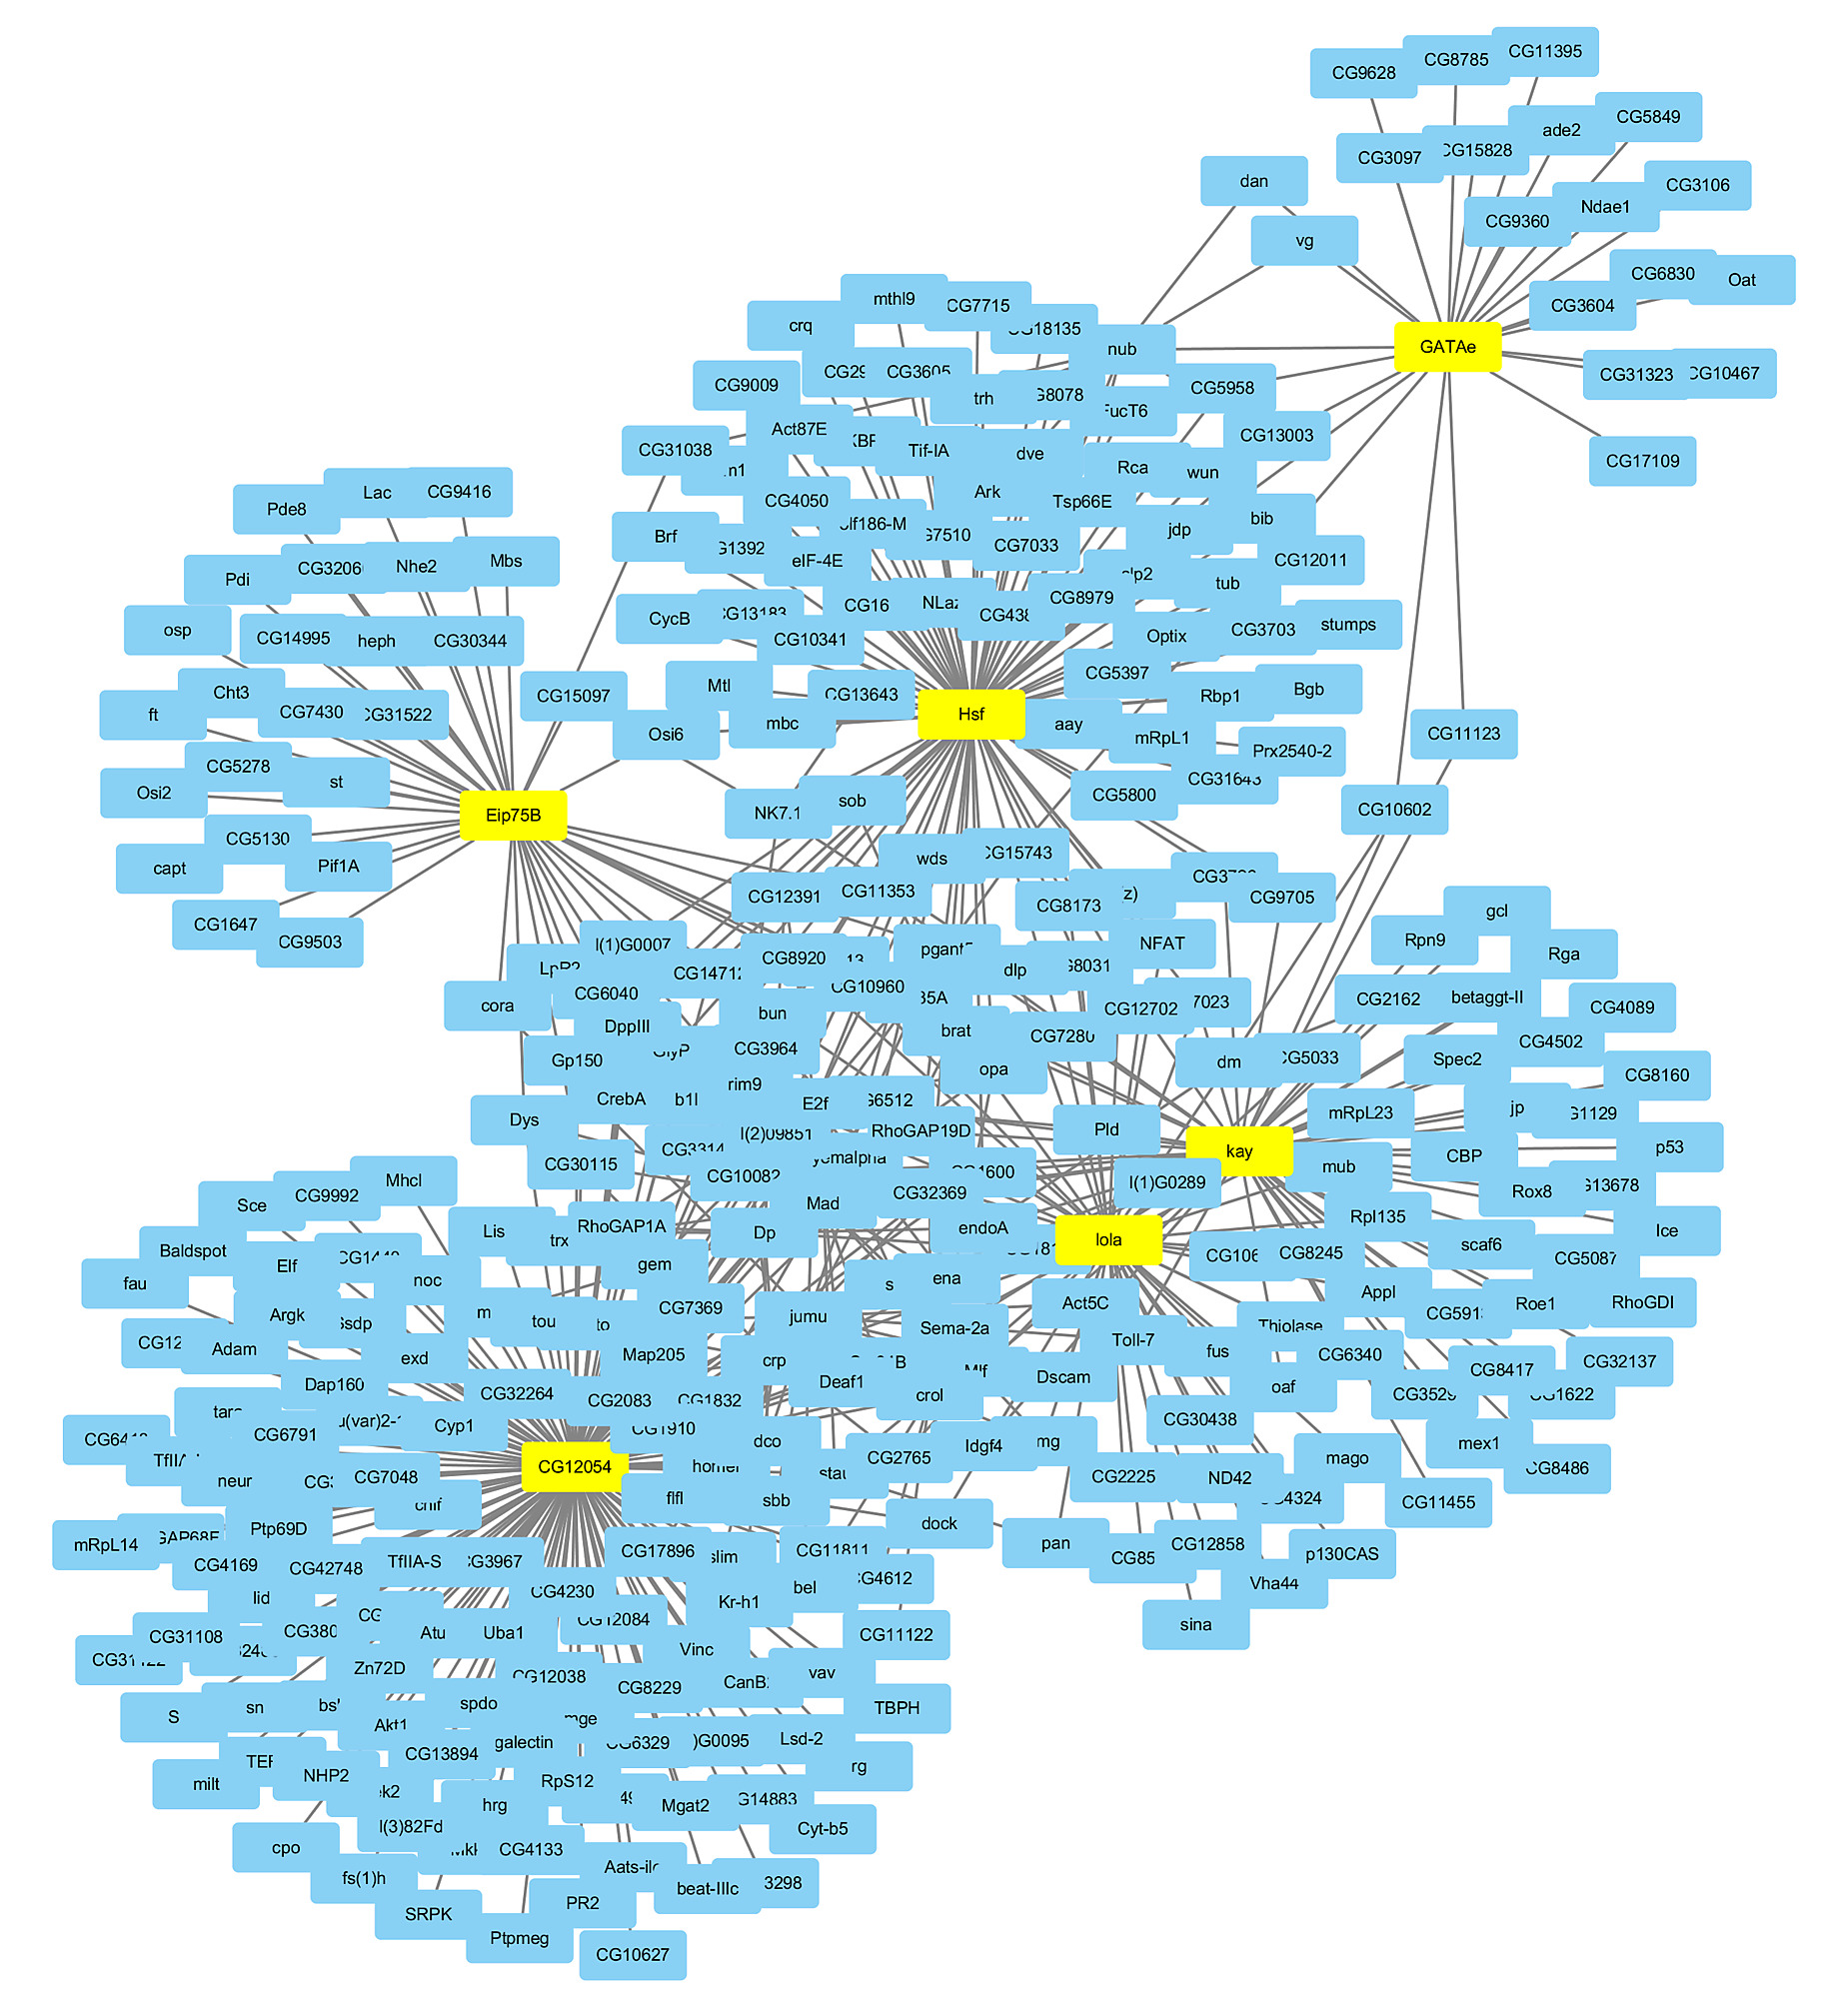
\includegraphics[scale=0.4]{bigdata.jpg}
\end{figure}
\end{frame}

\begin{frame}
\frametitle{Open Problems}
\begin{enumerate}
\item Gene regulatory networks are not fully understood \footnote{(Hartwell et al., 1999),(Ramons et al., 2010),(Shen-Orr et al. 2002)} 
\item biological  networks  are  often very large  \footnote{(Hallinan, J,2007)},
\item noisy data
\item GRNs are only indirectly observable  through  noisy  gene  expression  measurements.
\end{enumerate}
\end{frame}

\begin{frame}
\frametitle{The Role of Noise in biological systems}
We have 3 different type of noise in biological data:
\begin{enumerate}
\item Experimental noise (measurements)
\item Environmental noise 
\item Intrinsic noise (genes activity)
\end{enumerate}
\end{frame}

\begin{frame}
\frametitle{$1^o$ part of the PhD project - Filtering}
Deep learning:
\begin{enumerate}
\item Filtering data to reduce noise
\item Classification of communities of genes $\to$ Deep Neural Networks
\end{enumerate}
\end{frame}

\begin{frame}
\frametitle{$2^o$ part of the PhD project - The model}
\begin{enumerate}
\item Teoretical model for GRNs $\to$  Random Boolean Networks
\item multilayer network $\to$ interacting GRNs 

\end{enumerate}
\begin{figure}
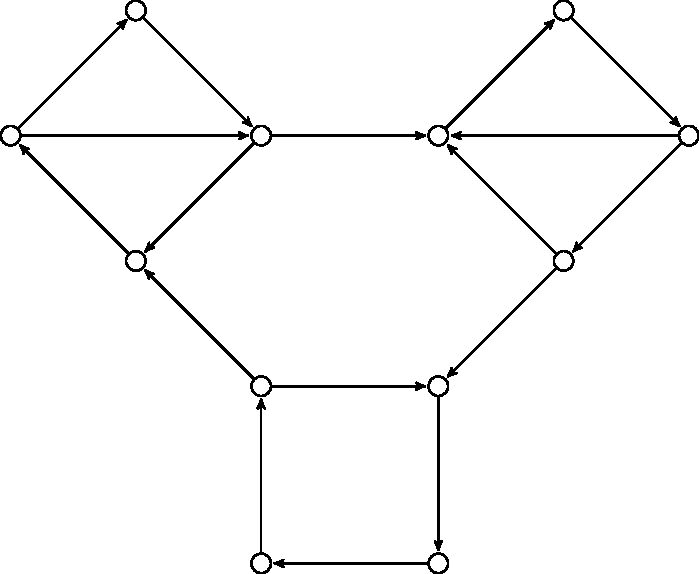
\includegraphics[scale = 0.5]{grn1.pdf}
\end{figure}
\end{frame}


\begin{frame}
\frametitle{The model}
A subnetwork hinibits the other: 
\begin{enumerate}
\item cellular differentiation 
\item cancer cells
\end {enumerate}
\begin{figure}[scale=0.5]
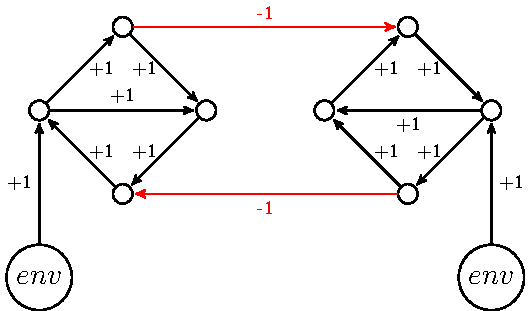
\includegraphics{grn.pdf}
\end{figure}
\end{frame}




\begin{frame}
\frametitle{Expected results}
\begin{enumerate}
\item Find a method to filter genomics data
\item Comparison of the model with experimental data
\item Determine the relation between the network structure and the dynamical properties of the system
\item Applications in genomics medicine

\end{enumerate}
\end{frame}





\end{document}

\begin{frame}
\frametitle{Conclusions}
The problems for this model are:
\begin{enumerate}
\item Classifying the equilibrium states in relation to their robustness with respect
the changes in the adjacency matrix
\item Understanding the representativity of the average dynamics: i.e. substituting
the adjacency matrix with an average matrix one highlights the dynamical
properties that are correctly described by the average system
\item Pointing out the existence of bifurcation phenomena so that it is possible to
divide the ensemble in different communities with similar dynamical behaviors.
\end{enumerate}
\end{frame}



